\documentclass[11pt,a4paper]{article}
\usepackage{ctex}
\usepackage{geometry}
\geometry{left=2.5cm,right=2.5cm,top=2.5cm,bottom=2.5cm}
\usepackage{amsmath}
\usepackage{amssymb}
\usepackage{graphicx}
\usepackage{tikz}
\usetikzlibrary{calc} % 引入用于几何坐标计算的库
\usepackage{eso-pic}

% 设置水印：一页三个斜着的，透明度调浅至 0.05
\AddToShipoutPictureBG{
  \begin{tikzpicture}[remember picture, overlay]
    \node[rotate=45, opacity=0.05, font=\fontsize{55}{55}\selectfont, text=gray] 
      at ([yshift=8cm]current page.center) {贺昱琪学习资料};
    \node[rotate=45, opacity=0.05, font=\fontsize{55}{55}\selectfont, text=gray] 
      at (current page.center) {贺昱琪学习资料};
    \node[rotate=45, opacity=0.05, font=\fontsize{55}{55}\selectfont, text=gray] 
      at ([yshift=-8cm]current page.center) {贺昱琪学习资料};
  \end{tikzpicture}
}

\begin{document}

\section*{贺昱琪八月第二周作业}

\begin{enumerate}

\item[1.] 黑板上有 $1, 3, 5, 7, \dots$ 若干个连续奇数，小明擦掉其中一个，剩下的数的和为 2020，则小明擦掉的数为\underline{\hspace{2cm}}。
\vspace{2cm}

\item[2.] 一个两位数，十位上的数字与个位上的数字和是 9，把十位上的数字与个位上的数字对调后，得到的数与原数的比是 $4:5$，则原来的两位数是\underline{\hspace{2cm}}。
\vspace{2cm}

\item[2.] (一半模型) 如图，$O$ 是长方形一条对角线的中点，图中已经标出两个三角形的面积为 3 和 4，那么阴影部分的一块直角三角形的面积是多少？
\hfill
    \begin{minipage}{0.3\textwidth}
        \centering
        
\includegraphics[width=\linewidth]{2.png}
    \end{minipage}
\vspace{2cm}
\item[3.] 已知一个直角三角形的三边长为 6cm，8cm，10cm，则该三角形的高为\underline{\hspace{2cm}}。
\vspace{2cm}

\item[3.] 已知等腰三角形一腰上的高和另一腰的夹角是 $25^\circ$，则这个等腰三角形的底角度数为\underline{\hspace{2cm}}。
\vspace{2cm}

\item[3.] (间隔发车) 甲城的车站总是以 20 分钟的时间间隔向乙城发车，甲、乙两城之间既有平路又有上坡和下坡，车辆(包括自行车)上坡和下坡的速度分别是平路上的 $80\%$ 和 $120\%$，有一名学生从乙城骑车去甲城，已知该学生平路上的骑车速度是汽车在平路上速度的四分之一，那么这位骑车的学生在平路、上坡、下坡时每隔多少分钟遇到一辆汽车？(8 分)
\vspace{3cm}

\item[4.] (10分) $A$、$B$ 两地之间是山路，相距 240 千米，其中一部分是上坡路，其余是下坡路。某人骑电动车从 $A$ 地到 $B$ 地，再沿原路返回，去时用了 11 小时，返回时用了 9 小时。已知下坡路每小时行驶 30 千米，那么上坡路每小时行驶多少千米？
\vspace{3cm}

\item[4.] 在长方形 $ABCD$ 中，已知两邻边 $AD=12$，$AB=5$，对角线 $AC=13$，$P$ 是 $AD$ 边上异于 $A$ 和 $D$ 的一个动点，过点 $P$ 分别向 $OA$，$OD$ 作垂线 $PE$、$PF$，那么 $PE+PF$ 有\underline{\hspace{1.5cm}}值 (最大、最小、定值)，这个值为\underline{\hspace{2cm}}。 
\begin{center}
\begin{tikzpicture}[scale=0.7]
  \coordinate (A) at (0,3); \coordinate (D) at (7,3);
  \coordinate (B) at (0,0); \coordinate (C) at (7,0);
  \draw[thick] (A) node[above left]{$A$} -- (D) node[above right]{$D$} -- (C) node[below right]{$C$} -- (B) node[below left]{$B$} -- cycle;
  \draw[thick] (A) -- (C); \draw[thick] (B) -- (D);
  \coordinate (O) at (3.5,1.5); \node[below] at (O) {$O$};
  \coordinate (P) at (2.5,3); \node[above] at (P) {$P$};
  \coordinate (E) at ($(A)!(P)!(C)$);
  \coordinate (F) at ($(D)!(P)!(B)$);
  \draw[thick, dashed] (P) -- (E) node[below left]{$E$};
  \draw[thick, dashed] (P) -- (F) node[below right]{$F$};
  \draw (E) ++(45:0.25) -- ++(-45:0.25) -- ++(-135:0.25);
  \draw (F) ++(135:0.25) -- ++(45:0.25) -- ++(-45:0.25);
  \node at (3.5, -1) {第 4 题图};
\end{tikzpicture}
\end{center}
\vspace{2cm}

\item[5.] (圆柱和圆锥的体积) 圆柱和圆锥的体积比是 $1:2$，底面积之比是 $2:3$，那么圆锥的高是圆柱高的\underline{\hspace{2cm}}倍。
\vspace{2cm}

\item[6.] 某人上山游玩，上山用了 120 分钟，沿原路下山，速度提高了 $\frac{1}{4}$，下山将用\underline{\hspace{2cm}}分钟。
\vspace{2cm}

\item[7.] 某会展中心大厅的 120 盏灯都是亮着的，每个灯都单独设有开关，现将开关按 $1\sim 120$ 编号。小王同学先按下编号为 3 的倍数的开关，然后再按下编号为 5 的倍数的开关，这时会展中心大厅中亮着的灯有\underline{\hspace{2cm}}盏。
\vspace{2cm}

\item[8.] 如图是圆柱被一个平面斜切后得到的几何体，请推算图中几何体的体积为\underline{\hspace{2cm}}。
\hfill
    \begin{minipage}{0.3\textwidth}
        \centering
        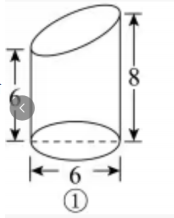
\includegraphics[width=\linewidth]{8.png}
    \end{minipage}
\vspace{2cm}
\vspace{2cm}

\item[9.] (钟表问题) 从 6 点到 7 点，时针和分针成直角的时间是\underline{\hspace{2cm}}时\underline{\hspace{2cm}}分和\underline{\hspace{2cm}}时\underline{\hspace{2cm}}分。
\vspace{2cm}

\item[10.] (差倍问题) 在一个三位数的前面加上数字 6，得到的四位数是原来三位数的 26 倍，原来的三位数是\underline{\hspace{2cm}}。
\vspace{2cm}

\item[10.] (相遇问题) $A,B$ 两地相距 950 米，甲、乙两人同时从 $A$ 地出发，往返 $A,B$ 两地跑步 30 分钟。甲跑步的速度是每分钟 40 米，乙跑步的速度是每分钟 150 米。在这段时间内他们相遇了数次，在第\underline{\hspace{2cm}}次相遇时他们离 $B$ 地的距离最近。
\vspace{3cm}

\item[11.] 如图，$\triangle ABC$ 的面积是 36 平方厘米，$AD = DE = EC$，$F$ 是 $BC$ 中点，$FG = GC$，阴影部分的面积是\underline{\hspace{2cm}}平方厘米。
\begin{center}
\begin{tikzpicture}[scale=1]
  \coordinate (B) at (0,0); \coordinate (C) at (6,0); \coordinate (A) at (2,3);
  \draw[thick] (A) node[above]{$A$} -- (B) node[below left]{$B$} -- (C) node[below right]{$C$} -- cycle;
  \coordinate (D) at ($(A)!0.333!(C)$); \node[above right] at (D) {$D$};
  \coordinate (E) at ($(A)!0.666!(C)$); \node[above right] at (E) {$E$};
  \coordinate (F) at ($(B)!0.5!(C)$); \node[below] at (F) {$F$};
  \coordinate (G) at ($(F)!0.5!(C)$); \node[below] at (G) {$G$};
  \fill[gray!60] (A) -- (B) -- (D) -- cycle;
  \fill[gray!60] (D) -- (F) -- (E) -- cycle;
  \fill[gray!60] (E) -- (G) -- (C) -- cycle;
  \draw[thick] (A) -- (B) -- (C) -- cycle;
  \draw[thick] (B) -- (D); \draw[thick] (D) -- (F); \draw[thick] (F) -- (E); \draw[thick] (E) -- (G);
  \node at (3, -1) {第 11 题图};
\end{tikzpicture}
\end{center}
\vspace{2cm}

\item[12.] 如图，小军用编号 1、2、3、4、5 的大小不同的正方形拼出一个长方形，则中间 5 号正方形的边长是\underline{\hspace{2cm}}厘米。
\hfill
    \begin{minipage}{0.3\textwidth}
        \centering
        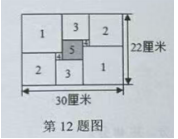
\includegraphics[width=\linewidth]{12.png}
    \end{minipage}
\vspace{2cm}
\vspace{2cm}

\item[13.] 桌上放有一张写有 61 的卡片，若从桌子的另一侧看去，却是 19。现在桌子上放着这样一道算术题：$89 + 16 + 69 + 6\square + \square 8 = 88$。甲、乙两位同学面对面坐在桌子两侧，而他们计算这道数学题的结果恰好相同，则两个方格中应填的数字和是\underline{\hspace{2cm}}。
\vspace{2cm}

\item[15.] (9分) 如图1是甲、乙两个圆柱形水槽的轴截面示意图，乙槽中有一圆柱形铁块放其中（圆柱形铁块的下底面完全落在水槽底面上）。现将甲槽中的水匀速注入乙槽。甲、乙两个水槽中水的深度 $y$ (厘米) 与注水时间 $x$ (分钟) 之间的关系如图2所示。根据图象提供的信息，解答下列问题：
\begin{center}
\begin{tikzpicture}[scale=0.4]
  % 图1: 甲
  \draw[thick] (0,4) -- (0,0) -- (3,0) -- (3,4);
  \draw[thick, dashed] (0,1.5) -- (3,1.5);
  \node at (1.5, -1) {甲};
  % 图1: 乙
  \draw[thick] (5,4) -- (5,0) -- (9,0) -- (9,4);
  \fill[gray!70] (6.5,0) rectangle (7.5, 2.5);
  \draw[thick, dashed] (5,0.5) -- (6.5,0.5); \draw[thick, dashed] (7.5,0.5) -- (9,0.5);
  \node at (7, -1) {乙};
  \node at (4.5, -2.5) {图1};
\end{tikzpicture}
\hspace{1cm}
\begin{tikzpicture}[scale=0.45]
  % 图2: 折线图
  \draw[->, thick] (0,0) -- (7,0) node[right]{$x$(分钟)};
  \draw[->, thick] (0,0) -- (0,7) node[above]{$y$(cm)};
  \draw[thick] (0, 4.5) node[left]{$14$} -- (6,0) node[above right]{$E$}; \node[above left] at (0, 4.5) {$D$};
  \draw[thick] (0, 0.6) node[left]{$2$} node[above left]{$A$} -- (4, 3.8) node[above left]{$B$} -- (6, 6) node[right]{$C$};
  \draw[dashed] (4,0) node[below]{$4$} -- (4,3.8);
  \draw[dashed] (0,3.8) node[left]{$12$} -- (4,3.8);
  \draw[dashed] (6,0) node[below]{$6$} -- (6,6);
  \draw[dashed] (0,6) node[left]{$19$} -- (6,6);
  \node at (3, -2.5) {图2};
\end{tikzpicture}
\end{center}
\begin{itemize}
    \item[(1)] 图2中折线 $ABC$ 表示\underline{\hspace{2cm}}槽中的深度与注水时间之间的关系，线段 $DE$ 表示\underline{\hspace{2cm}}槽中的深度与注水时间之间的关系 (以上两空均填“甲”或“乙”)，点 $B$ 的纵坐标表示的实际意义是\underline{\hspace{4cm}}。
    \vspace{1.5cm}
    \item[(2)] 注水多长时间时，甲、乙两个水槽中的水深相同？
    \vspace{2.5cm}
    \item[(3)] 若乙槽底面积为 36 平方厘米 (壁厚不计)，求乙槽中铁块的体积。
    \vspace{2.5cm}
\end{itemize}

\item[16.] (10分) 如图1，在长方形 $ABCD$ 中，$AB=12$ 厘米，$BC=6$ 厘米。点 $P$ 沿 $AB$ 边从点 $A$ 开始向点 $B$ 以 2 厘米/秒的速度移动；点 $Q$ 沿 $DA$ 边从点 $D$ 开始向点 $A$ 以 1 厘米/秒的速度移动。如果 $P$、$Q$ 同时出发，用 $t$ (秒) 表示移动的时间，那么：
\begin{center}
\begin{tikzpicture}[scale=0.6]
  \draw[thick] (0,0) node[below left]{$A$} -- (5,0) node[below right]{$B$} -- (5,3) node[above right]{$C$} -- (0,3) node[above left]{$D$} -- cycle;
  \draw[thick] (0,1.5) node[left]{$Q$} -- (1.5,0) node[below]{$P$};
  \draw[->] (0,3) -- (0,2); \draw[->] (0,0) -- (1,0);
  \node at (2.5, -1) {图1};
\end{tikzpicture}
\hspace{2cm}
\begin{tikzpicture}[scale=0.6]
  \draw[thick] (0,0) node[below left]{$A$} -- (5,0) node[below right]{$B$} -- (5,3) node[above right]{$C$} -- (0,3) node[above left]{$D$} -- cycle;
  \draw[thick] (0,1.5) node[left]{$Q$} -- (3.5,0) node[below]{$P$};
  \draw[->] (0,3) -- (0,2); \draw[->] (0,0) -- (2.5,0);
  \node at (2.5, -1) {图2};
\end{tikzpicture}
\end{center}
\begin{itemize}
    \item[(1)] $DQ=$\underline{\hspace{2cm}}厘米，$AP=$\underline{\hspace{2cm}}厘米 (用含 $t$ 的代数式表示)
    \vspace{1.5cm}
    \item[(2)] 如图1，当 $t=$\underline{\hspace{2cm}}秒时，线段 $AQ$ 与线段 $AP$ 相等？
    \vspace{2cm}
    \item[(3)] 如图2，$P$、$Q$ 到达 $B$、$A$ 后继续运动，$P$ 点到达 $C$ 点后都停止运动。当 $t$ 为何值时，线段 $AQ$ 的长等于线段 $CP$ 的长的一半。
    \vspace{3cm}
\end{itemize}

\item[16.] 三枚半径为 1cm 的圆形硬币相互紧靠着平放在桌面上，让一枚硬币沿着它们的外轮廓滚过后回到原来的位置，那么与原 $A$ 点重合的点是哪个点？硬币圆心运动轨迹的周长是多少厘米？(结果保留 $\pi$)
\begin{center}
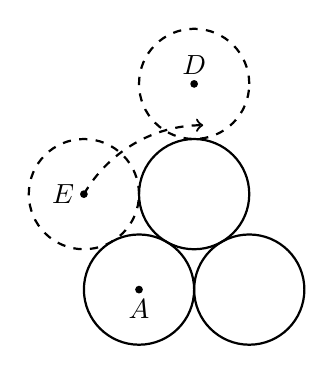
\begin{tikzpicture}[scale=0.7]
  \coordinate (O1) at (0,0); \draw[thick] (O1) circle (1); \fill (O1) circle (2pt) node[below]{$A$};
  \coordinate (O2) at (2,0); \draw[thick] (O2) circle (1);
  \coordinate (O3) at (1,1.732); \draw[thick] (O3) circle (1);
  \coordinate (P1) at (-1, 1.732); \draw[thick, dashed] (P1) circle (1); \fill (P1) circle (2pt) node[left]{$E$};
  \coordinate (P2) at (1, 3.732); \draw[thick, dashed] (P2) circle (1); \fill (P2) circle (2pt) node[above]{$D$};
  \draw[->, thick, dashed] (P1) arc (150:90:2.5);
\end{tikzpicture}
\end{center}
\vspace{3cm}

\item[16.] (商品利润) 某收音机成本 72 元，原来按定价出售，每天可售 100 个，每件利润为成本的 $25\%$，后来按定价打九折出售，每天销售量提高到原来的 2.5 倍。照这样计算，每天的利润比原来增加多少元？(7 分)
\vspace{3cm}

\item[17.] 一水箱有甲、乙、丙三根进水管，如果只打开甲、丙两管，甲管注入 30 吨水时，水箱已满；如果只打开乙、丙两管，乙管注入 40 吨水时，水箱才满。已知乙管每分钟注水量是甲管的 1.5 倍。请问：该水箱注满时可容纳多少吨水？
\vspace{3cm}

\item[18.] 单位的职工到郊外植树，其中有男职工，也有女职工，并且有 $\frac{1}{3}$ 的职工各带一个孩子参加。男职工每人种 13 棵树，女职工每人种 10 棵树，每个孩子都种 6 棵树，他们一共种了 216 棵树，那么其中有多少名男职工？
\vspace{3cm}

\item[19.] 某商品 76 件，出售给 33 位顾客，每位顾客最多买三件。如果买一件按原定价，买两件降价 $10\%$，买三件降价 $20\%$，最后结算，平均每件恰好按原定价的 $85\%$ 出售。那么买三件的顾客有多少人？
\vspace{3cm}

\item[20.] (工程问题) 有 $A$，$B$ 两个仓库，$A$ 仓库的货物是 $B$ 仓库的 2 倍，搬运完 $A$ 仓库的货物，甲单干需\underline{\hspace{1.5cm}}小时；搬运完 $B$ 仓库的货物，乙单干需要 24 小时，丙单干需要 12 小时。刚开始甲搬运 $A$ 仓库，乙搬运 $B$ 仓库，丙先帮甲，后来丙又去帮乙，直到最后两个仓库的货物同时搬完，则丙帮了甲几个小时？(7 分)
\vspace{3cm}

\item[22.] 有一个正方形和两个等边三角形的位置如图所示，若 $\angle 3 = 50^\circ$，那么 $\angle 1 + \angle 2$ 等于多少度？
\hfill
    \begin{minipage}{0.3\textwidth}
        \centering
        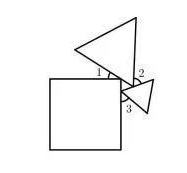
\includegraphics[width=\linewidth]{22.png}
    \end{minipage}
\vspace{2cm}
\vspace{3cm}

\item[计算题] 
\begin{itemize}
    \item[(1)] $2\frac{3}{5} \times \frac{3}{4} - \frac{2}{5} \times \frac{3}{4}$
    \vspace{2cm}
    \item[(2)] $3.64 \times \frac{1}{4} + 4.36 \times 0.25$
    \vspace{2cm}
    \item[(3)] $\left[7\frac{1}{2} - \left(1\frac{5}{8} - \frac{1}{2} \times \frac{3}{4}\right)\right] \div 3$
    \vspace{2cm}
    \item[(4)] $\left[\frac{8}{9} \times \left(\frac{4}{5} - 0.35\right) + 30\%\right] \div \frac{3}{5}$
    \vspace{2cm}
\end{itemize}

\item[二、计算] 
\begin{itemize}
    \item[1.] $6.8 \times \frac{8}{25} + 0.32 \times 4.2 - 8 \div 25$
    \vspace{3cm}
    \item[2.] $0.7 \times 1\frac{2}{11} - 6.6 \times \frac{3}{7} - 2.2 \div \frac{7}{3} + 0.7 \times \frac{9}{11} + 3.3 \div \frac{7}{8}$
    \vspace{3cm}
\end{itemize}

\end{enumerate}

\end{document}